% Options for packages loaded elsewhere
\PassOptionsToPackage{unicode}{hyperref}
\PassOptionsToPackage{hyphens}{url}
\PassOptionsToPackage{dvipsnames,svgnames,x11names}{xcolor}
%
\documentclass[
  a4paper,
]{article}

\usepackage{amsmath,amssymb}
\usepackage{iftex}
\ifPDFTeX
  \usepackage[T1]{fontenc}
  \usepackage[utf8]{inputenc}
  \usepackage{textcomp} % provide euro and other symbols
\else % if luatex or xetex
  \usepackage{unicode-math}
  \defaultfontfeatures{Scale=MatchLowercase}
  \defaultfontfeatures[\rmfamily]{Ligatures=TeX,Scale=1}
\fi
\usepackage{lmodern}
\ifPDFTeX\else  
    % xetex/luatex font selection
\fi
% Use upquote if available, for straight quotes in verbatim environments
\IfFileExists{upquote.sty}{\usepackage{upquote}}{}
\IfFileExists{microtype.sty}{% use microtype if available
  \usepackage[]{microtype}
  \UseMicrotypeSet[protrusion]{basicmath} % disable protrusion for tt fonts
}{}
\makeatletter
\@ifundefined{KOMAClassName}{% if non-KOMA class
  \IfFileExists{parskip.sty}{%
    \usepackage{parskip}
  }{% else
    \setlength{\parindent}{0pt}
    \setlength{\parskip}{6pt plus 2pt minus 1pt}}
}{% if KOMA class
  \KOMAoptions{parskip=half}}
\makeatother
\usepackage{xcolor}
\usepackage[top=2.54cm,right=2.54cm,bottom=2.54cm,left=2.54cm]{geometry}
\setlength{\emergencystretch}{3em} % prevent overfull lines
\setcounter{secnumdepth}{-\maxdimen} % remove section numbering
% Make \paragraph and \subparagraph free-standing
\ifx\paragraph\undefined\else
  \let\oldparagraph\paragraph
  \renewcommand{\paragraph}[1]{\oldparagraph{#1}\mbox{}}
\fi
\ifx\subparagraph\undefined\else
  \let\oldsubparagraph\subparagraph
  \renewcommand{\subparagraph}[1]{\oldsubparagraph{#1}\mbox{}}
\fi

\usepackage{color}
\usepackage{fancyvrb}
\newcommand{\VerbBar}{|}
\newcommand{\VERB}{\Verb[commandchars=\\\{\}]}
\DefineVerbatimEnvironment{Highlighting}{Verbatim}{commandchars=\\\{\}}
% Add ',fontsize=\small' for more characters per line
\newenvironment{Shaded}{}{}
\newcommand{\AlertTok}[1]{\textcolor[rgb]{1.00,0.33,0.33}{\textbf{#1}}}
\newcommand{\AnnotationTok}[1]{\textcolor[rgb]{0.42,0.45,0.49}{#1}}
\newcommand{\AttributeTok}[1]{\textcolor[rgb]{0.84,0.23,0.29}{#1}}
\newcommand{\BaseNTok}[1]{\textcolor[rgb]{0.00,0.36,0.77}{#1}}
\newcommand{\BuiltInTok}[1]{\textcolor[rgb]{0.84,0.23,0.29}{#1}}
\newcommand{\CharTok}[1]{\textcolor[rgb]{0.01,0.18,0.38}{#1}}
\newcommand{\CommentTok}[1]{\textcolor[rgb]{0.42,0.45,0.49}{#1}}
\newcommand{\CommentVarTok}[1]{\textcolor[rgb]{0.42,0.45,0.49}{#1}}
\newcommand{\ConstantTok}[1]{\textcolor[rgb]{0.00,0.36,0.77}{#1}}
\newcommand{\ControlFlowTok}[1]{\textcolor[rgb]{0.84,0.23,0.29}{#1}}
\newcommand{\DataTypeTok}[1]{\textcolor[rgb]{0.84,0.23,0.29}{#1}}
\newcommand{\DecValTok}[1]{\textcolor[rgb]{0.00,0.36,0.77}{#1}}
\newcommand{\DocumentationTok}[1]{\textcolor[rgb]{0.42,0.45,0.49}{#1}}
\newcommand{\ErrorTok}[1]{\textcolor[rgb]{1.00,0.33,0.33}{\underline{#1}}}
\newcommand{\ExtensionTok}[1]{\textcolor[rgb]{0.84,0.23,0.29}{\textbf{#1}}}
\newcommand{\FloatTok}[1]{\textcolor[rgb]{0.00,0.36,0.77}{#1}}
\newcommand{\FunctionTok}[1]{\textcolor[rgb]{0.44,0.26,0.76}{#1}}
\newcommand{\ImportTok}[1]{\textcolor[rgb]{0.01,0.18,0.38}{#1}}
\newcommand{\InformationTok}[1]{\textcolor[rgb]{0.42,0.45,0.49}{#1}}
\newcommand{\KeywordTok}[1]{\textcolor[rgb]{0.84,0.23,0.29}{#1}}
\newcommand{\NormalTok}[1]{\textcolor[rgb]{0.14,0.16,0.18}{#1}}
\newcommand{\OperatorTok}[1]{\textcolor[rgb]{0.14,0.16,0.18}{#1}}
\newcommand{\OtherTok}[1]{\textcolor[rgb]{0.44,0.26,0.76}{#1}}
\newcommand{\PreprocessorTok}[1]{\textcolor[rgb]{0.84,0.23,0.29}{#1}}
\newcommand{\RegionMarkerTok}[1]{\textcolor[rgb]{0.42,0.45,0.49}{#1}}
\newcommand{\SpecialCharTok}[1]{\textcolor[rgb]{0.00,0.36,0.77}{#1}}
\newcommand{\SpecialStringTok}[1]{\textcolor[rgb]{0.01,0.18,0.38}{#1}}
\newcommand{\StringTok}[1]{\textcolor[rgb]{0.01,0.18,0.38}{#1}}
\newcommand{\VariableTok}[1]{\textcolor[rgb]{0.89,0.38,0.04}{#1}}
\newcommand{\VerbatimStringTok}[1]{\textcolor[rgb]{0.01,0.18,0.38}{#1}}
\newcommand{\WarningTok}[1]{\textcolor[rgb]{1.00,0.33,0.33}{#1}}

\providecommand{\tightlist}{%
  \setlength{\itemsep}{0pt}\setlength{\parskip}{0pt}}\usepackage{longtable,booktabs,array}
\usepackage{calc} % for calculating minipage widths
% Correct order of tables after \paragraph or \subparagraph
\usepackage{etoolbox}
\makeatletter
\patchcmd\longtable{\par}{\if@noskipsec\mbox{}\fi\par}{}{}
\makeatother
% Allow footnotes in longtable head/foot
\IfFileExists{footnotehyper.sty}{\usepackage{footnotehyper}}{\usepackage{footnote}}
\makesavenoteenv{longtable}
\usepackage{graphicx}
\makeatletter
\def\maxwidth{\ifdim\Gin@nat@width>\linewidth\linewidth\else\Gin@nat@width\fi}
\def\maxheight{\ifdim\Gin@nat@height>\textheight\textheight\else\Gin@nat@height\fi}
\makeatother
% Scale images if necessary, so that they will not overflow the page
% margins by default, and it is still possible to overwrite the defaults
% using explicit options in \includegraphics[width, height, ...]{}
\setkeys{Gin}{width=\maxwidth,height=\maxheight,keepaspectratio}
% Set default figure placement to htbp
\makeatletter
\def\fps@figure{htbp}
\makeatother

\usepackage{booktabs}
\usepackage{longtable}
\usepackage{array}
\usepackage{multirow}
\usepackage{wrapfig}
\usepackage{float}
\usepackage{colortbl}
\usepackage{pdflscape}
\usepackage{tabu}
\usepackage{threeparttable}
\usepackage{threeparttablex}
\usepackage[normalem]{ulem}
\usepackage{makecell}
\usepackage{xcolor}
% Preámbulo
\usepackage{comment} % Permite comentar secciones del código
\usepackage{marvosym} % Agrega símbolos adicionales
\usepackage{graphicx} % Permite insertar imágenes
\usepackage{mathptmx} % Fuente de texto matemática
\usepackage{amssymb} % Símbolos adicionales de matemáticas
\usepackage{lipsum} % Crea texto aleatorio
\usepackage{float} % Control de posiciones de figuras y tablas
\usepackage{rotating} % Rotación de elementos
\usepackage{multirow} % Celdas combinadas en tablas
\usepackage{tabularx} % Tablas con ancho de columna ajustable
\usepackage{mdframed} % Marcos alrededor de elementos flotantes

% Series de tiempo
\usepackage{booktabs}


% Configuración adicional

\makeatletter
\makeatother
\makeatletter
\makeatother
\makeatletter
\@ifpackageloaded{caption}{}{\usepackage{caption}}
\AtBeginDocument{%
\ifdefined\contentsname
  \renewcommand*\contentsname{Tabla de contenidos}
\else
  \newcommand\contentsname{Tabla de contenidos}
\fi
\ifdefined\listfigurename
  \renewcommand*\listfigurename{Listado de Figuras}
\else
  \newcommand\listfigurename{Listado de Figuras}
\fi
\ifdefined\listtablename
  \renewcommand*\listtablename{Listado de Tablas}
\else
  \newcommand\listtablename{Listado de Tablas}
\fi
\ifdefined\figurename
  \renewcommand*\figurename{Figura}
\else
  \newcommand\figurename{Figura}
\fi
\ifdefined\tablename
  \renewcommand*\tablename{Tabla}
\else
  \newcommand\tablename{Tabla}
\fi
}
\@ifpackageloaded{float}{}{\usepackage{float}}
\floatstyle{ruled}
\@ifundefined{c@chapter}{\newfloat{codelisting}{h}{lop}}{\newfloat{codelisting}{h}{lop}[chapter]}
\floatname{codelisting}{Listado}
\newcommand*\listoflistings{\listof{codelisting}{Listado de Listados}}
\makeatother
\makeatletter
\@ifpackageloaded{caption}{}{\usepackage{caption}}
\@ifpackageloaded{subcaption}{}{\usepackage{subcaption}}
\makeatother
\makeatletter
\@ifpackageloaded{tcolorbox}{}{\usepackage[skins,breakable]{tcolorbox}}
\makeatother
\makeatletter
\@ifundefined{shadecolor}{\definecolor{shadecolor}{rgb}{.97, .97, .97}}
\makeatother
\makeatletter
\makeatother
\makeatletter
\makeatother
\ifLuaTeX
\usepackage[bidi=basic]{babel}
\else
\usepackage[bidi=default]{babel}
\fi
\babelprovide[main,import]{spanish}
% get rid of language-specific shorthands (see #6817):
\let\LanguageShortHands\languageshorthands
\def\languageshorthands#1{}
\ifLuaTeX
  \usepackage{selnolig}  % disable illegal ligatures
\fi
\usepackage[]{biblatex}
\addbibresource{../../../../references.bib}
\IfFileExists{bookmark.sty}{\usepackage{bookmark}}{\usepackage{hyperref}}
\IfFileExists{xurl.sty}{\usepackage{xurl}}{} % add URL line breaks if available
\urlstyle{same} % disable monospaced font for URLs
\hypersetup{
  pdftitle={Notas de Clase Series de Tiempo},
  pdfauthor={Edison Achalma},
  pdflang={es},
  colorlinks=true,
  linkcolor={blue},
  filecolor={Maroon},
  citecolor={Blue},
  urlcolor={Blue},
  pdfcreator={LaTeX via pandoc}}

\title{Notas de Clase Series de Tiempo}
\usepackage{etoolbox}
\makeatletter
\providecommand{\subtitle}[1]{% add subtitle to \maketitle
  \apptocmd{\@title}{\par {\large #1 \par}}{}{}
}
\makeatother
\subtitle{Descubre cómo seleccionar hardware, descargar la imagen ISO y
preparar los medios de instalación. Exploraremos opciones para probar o
instalar Linux en tu equipo.}
\author{Edison Achalma}
\date{2023-08-27}

\begin{document}
\maketitle
\ifdefined\Shaded\renewenvironment{Shaded}{\begin{tcolorbox}[enhanced, frame hidden, boxrule=0pt, sharp corners, borderline west={3pt}{0pt}{shadecolor}, interior hidden, breakable]}{\end{tcolorbox}}\fi

\hypertarget{elementos-de-ecuaciones-en-diferencia}{%
\section{Elementos de Ecuaciones en
Diferencia}\label{elementos-de-ecuaciones-en-diferencia}}

\hypertarget{a-ecuaciones-en-diferencia-para-procesos-deterministas}{%
\subsection{a) Ecuaciones en Diferencia para procesos
deterministas}\label{a-ecuaciones-en-diferencia-para-procesos-deterministas}}

En el capítulo previo se hizo una introducción al concepto de series de
tiempo. En este Capítulo se pretende desarrollar la construcción de los
procesos generadores de datos de las series de tiempo. En un sentido más
formal, se expondrá que las series de tiempo se pueden considerar como
una secuencia de variables aleatorias.

Para tales efectos, se desarrollará una introducción al concepto de
ecuaciones en diferencia. Así, las preguntas que se pretende responder
son:

\begin{enumerate}
\def\labelenumi{\alph{enumi}.}
\item
  ¿Cuál es la solución de la ecuación en diferencia que se estudia?
\item
  ¿Cuáles son las condiciones para que un proceso estocástico,
  representado mediante una ecuación en diferencia, llegue a alcanzar un
  punto de equilibrio en el largo plazo?
\end{enumerate}

El término de \emph{ecuación en diferencia} sirve para denominar un
proceso similar o equivalente dentro de las ecuaciones diferenciales,
dentro del cual se consideran a un conjunto de variables que están en
función del tiempo. Así, si consideramos al tiempo como una variable
continua, es decir, consideramos una variable \(Z(t)\), podemos expresar
las siguientes expresiones para la ecuación diferencial:

\begin{equation}\protect\hypertarget{eq-eqDiff}{}{
\frac{dZ(t)}{dt}; \frac{d^2Z(t)}{dt^2}; \ldots; \frac{d^kZ(t)}{dt^k}
}\label{eq-eqDiff}\end{equation}

Por otro lado, suponiendo el caso del tiempo en forma discreta, es
decir, con \(t = \ldots, -2, -1, 0, 1, 2, \ldots\), entonces el
comportamiento de la serie de variables dadas por \(Z_t\), la cual se
puede expresar como:

\begin{equation}\protect\hypertarget{eq-Diff1}{}{
\Delta Z_t; \Delta^2 Z_t; \ldots; \Delta^k Z_t
}\label{eq-Diff1}\end{equation}

Observemos que una forma técnicamente más correcta es escribir las
expresiones anteriores como:

\begin{equation}\protect\hypertarget{eq-Diff2}{}{
\frac{\Delta Z_t}{\Delta t}; \frac{\Delta^2 Z_t}{\Delta t^2}; \ldots; \frac{\Delta^k Z_t}{\Delta t^k}
}\label{eq-Diff2}\end{equation}

No obstante, no pasa desapercibido que \(\Delta t = 1\), por lo que
resultan equivalentes ambos conjuntos de expresiones
(Ecuación~\ref{eq-Diff1}) y (Ecuación~\ref{eq-Diff2}).

\hypertarget{ecuaciones-en-diferencia-lineales-de-primer-orden}{%
\subsubsection{Ecuaciones en Diferencia Lineales de Primer
Orden}\label{ecuaciones-en-diferencia-lineales-de-primer-orden}}

El primer caso que se suele estudiar en relación a Ecuaciones en
Diferencia es el de las Ecuaciones en Diferencia Lineales de Primer
Orden. Al respecto, al igual que en el caso continúo, las variaciones de
la variable \(Z_t\) se pueden expresar como se ilustra en el siguiente
ejemplo. Consideremos la siguiente ecuación:

\begin{equation}\protect\hypertarget{eq-EDPO}{}{
Z_t = a_0 + a_1 Z_{t-1}
}\label{eq-EDPO}\end{equation}

Donde, \(t = \ldots, -2, -1, 0, 1, 2, \ldots\), y \(a_0\) y
\(a_1 \neq 0\) son números reales constantes. De
(Ecuación~\ref{eq-EDPO}) podememos despejar la variable \(Z_{t-1}\) y
obtener una forma de ecuación en diferencia:

\begin{equation}\protect\hypertarget{eq-EDPO2}{}{
Z_t - a_1 Z_{t-1} = a_0
}\label{eq-EDPO2}\end{equation}

Ahora denotemos a \(L Z_t = Z_{t-1}\), es decir, mediante el operador
\(L\) se puede rezagar una variable dada. En general, podemos decir que
el operador tiene dos propiedades, la primera es que es lineal en el
sentido de que abre sumas y saca escalares como se muestra en la
siguiente expresión para el caso de un (1) rezago:

\begin{equation}\protect\hypertarget{eq-E1Lag}{}{
L(\alpha Z_{t} + \beta) = \alpha Z_{t-1} + \beta
}\label{eq-E1Lag}\end{equation}

Donde \(\alpha, \beta \in \mathbb{R}\) y \(\alpha, \beta \neq 0\). Otro
reesultado implícito en esta primera propiedad es que el operador rezago
aplicado a cualquier escalar dará como resultado el escalar, puesto que
este es una constante sin importa el momento \(t\) en el cual se
encuentre la variable \(Z\).

La segunda propiedad del operador es que se puede aplicar de forma
consecutiva a una misma variable. Es decir,
\(L ( Z_{t-1}) = L L Z_{t} = L^2 Z_{t}\), por lo que en general
tendremos: \(L^p Z_t = Z_{t-p}\) (con \(p \in \mathbb{Z}\)). Así, en el
caso de p rezagos la propiedad de linealidad del operador rezago será:

\begin{equation}\protect\hypertarget{eq-LinProp}{}{
L^p (\alpha Z_{t} + \beta) = \alpha Z_{t-p} + \beta
}\label{eq-LinProp}\end{equation}

Dicho lo anterior podemos escribir la solución general de
(Ecuación~\ref{eq-EDPO2}) como:

\begin{align}
Z_t - a_1 L Z_t & = a_0 \nonumber \\
(1 - a_1 L)Z_t & = a_0 \nonumber \\
Z_t & = a_0 \frac{1}{1 - a_1 L} + s a^t_1 \nonumber \\
Z_t & = a_0 \frac{1}{1 - a_1} + s a^t_1
\end{align} \{\#eq-PROC01\}

Donde \(a_1 \neq 1\) y \(t = \ldots, -2, -1, 0, 1, 2, \ldots\). Notése
que la aplicación del operador rezago \(L\) a la constante \(a_1\) dará
como resultado el valor de la misma constante, ya que ésta no depende
del momento \(t\) en el cuál observemos a la variable \(Z_t\). En la
(\textbf{?@eq-PROC01}) se adiciona un término \(s a^t_1\) que permite
ubicar la trayectoria inicial de la solución de la ecuación. El
componente no significa un cambio respecto de la
(Ecuación~\ref{eq-EDPO2}) original, ya que si buscaramos reconstruir a
ésta ecuación tendríamos:

\begin{align}
(1 - a_1 L) s a^t_1 & = s a^t_1 - a_1 s L a^{t}\_1 \nonumber \\
& = s a^t_1 - a_1 s a^{t - 1}\_1 \nonumber \\
& = s a^t_1 - s a^t_1 \nonumber \\
& = 0 \nonumber
\end{align}

La (\textbf{?@eq-PROC01}) se suele interpretar como la solución de largo
plazo. Ahora demostraremos por qué es cierta la ecuación y discutiremos
algunas condiciones que se deben observar en esta solución para que sea
una solución convergente. No obstante, primero discutiremos un método
indirecto e incompleto para demostrar el resultado, dicho método es
conocido como el método iterativo. Plantearemos las siguientes
ecuaciones partículares donde suponemos la existencia del valor inicial
\(Z_0\) del proceso:

\begin{equation*}
Z_1 = a_0 + a_1 Z_0
\end{equation*}

\begin{align*}
Z_2 & = a_0 + a_1 Z_1 \\
& = a_0 + a_1 (a_0 + a_1 Z_0) \\
& = a_0 + a_0 a_1 + a^2_1 Z_0 \\
& = a_0 (1 + a_1) + a^2_1 Z_0
\end{align*}

\begin{align*}
Z_3 & = a_0 + a_1 Z_2 \\
& = a_0 + a_1 (a_0 + a_0 a_1 + a^2_1 Z_0) \\
& = a_0 + a_0 a_1 + a_0 a^2_1 + a^3_1 Z_0 \\
& = a_0 (1 + a_1 + a^2_1) + a^3_1 Z_0
\end{align*}

De lo anterior se puede inferir que el método iterativo convergerá hacia
una expresión como la siguiente en el momento \(t\):

\begin{align}
Z*t & = a_0 + a_1 Z*{t-1} \nonumber \\
& = a*0 (1 + a_1 + a^2_1 + \ldots + a^{t-1}\_1) + a^t_1 Z_0 \nonumber \\
& = a_0 \sum^{t-1}*{i = 0}{a^i_1} + a^t_1 Z_0
\end{align} \{\#eq-SUM\}

Donde, es necesario que en la (\textbf{?@eq-SUM}) se cumpla que
\(\lvert{a_1}\lvert < 1\) para que la suma sea convergente --más
adelante detallaremos esta afirmación--. A este tipo de ecuaciones se
les puede denominar como lineales. Esto en razón de que ningún término
de la variable \(Z\) aparce elevado a ninguna potencia distinta a 1.
También, son de primer orden, ya que el rezago de la variable \(Z\) es
sólo de un período.

En adelante trabajaremos con ecuaciones en las que la variable \(Z\) se
encuentra rezagada en cualquiera de los siguientes casos:

\begin{equation}\protect\hypertarget{eq-SUM0}{}{
Z_t, Z_{t-1}, Z_{t-2}, Z_{t-3}, \ldots, Z_{t-p}, \ldots
}\label{eq-SUM0}\end{equation}

Por lo que diremos que en adelante el curso versará sobre ecuaciones en
diferencia lineales y de cualquier orden \(p\).

Retomando la (\textbf{?@eq-SUM}) y considerando la parte de la suma de
los términos de \(a^i_1\), de tal forma que buscaremos dar una expresión
más compresible a dicho término. Definamos la siguiente expresión como:

\begin{equation}\protect\hypertarget{eq-St1}{}{
S_{t-1} = \sum^{t-1}_{i = 0}{a^i_1}
}\label{eq-St1}\end{equation}

Por lo tanto, \(S_t\) estaría dado por la siguiente expresión:

\begin{align}
S*{t} & = a_1 \sum^{t-1}*{i = 0}{a^i*1} \nonumber \\
& = a_1 (1 + a_1 + a^2_1 + \ldots + a^{t-1}\_1) \nonumber \\
& = a_1 + a^2_1 + a^3_1 + \ldots + a^{t}\_1 \nonumber \\
& = a_1 S*{t-1}
\end{align} \{\#eq-St\}

Tomando los dos resultados de la (Ecuación~\ref{eq-St1}) y
(\textbf{?@eq-St}), podemos expresar que si a \(S_{t-1}\) le restamos
\(S_t\), y desarrollando ambos lados de la ecuación anterior podemos
obtener:

\begin{align}
S*{t-1} - a_1 S*{t-1} & = S*{t-1} - S*{t} \nonumber \\
(1 - a*1) S*{t-1} & = (1 + a*1 + a^2_1 + \ldots + a^{t-1}\_1) - (a_1 + a^2_1 + a^3_1 + \ldots + a^{t}\_1) \nonumber \\
(1 - a_1) S*{t-1} & = 1 - a^{t}\_1 \nonumber
\end{align}

Así, podemos concluir que:

\begin{equation}\protect\hypertarget{eq-SUM2}{}{
S_{t-1} = \frac{1 - a^{t}_1}{1 - a_1}
}\label{eq-SUM2}\end{equation}

Conjuntando éste último resultado de la ecuación
(Ecuación~\ref{eq-SUM2}) con la ecuación (\textbf{?@eq-SUM}) tenemos la
siguiente solución por el método de iteración:

\begin{equation}\protect\hypertarget{eq-SOLITER}{}{
Z_t = a_0 \left( \frac{1 - a^{t}_1}{1 - a_1} \right) + a^t_1 Z_0
}\label{eq-SOLITER}\end{equation}

De esta forma la (Ecuación~\ref{eq-SOLITER}) es una solición para la
(\textbf{?@eq-SUM}), que es una ecuación de un proceso de una Ecuación
en Diferencia plantenado en la (Ecuación~\ref{eq-EDPO}). Está solución
aún no es general, en el sentido de que sea válida para cualquiel tipo
de proceso: convergente o divergente. Dicha convergencia o divengencia
estará determinada por el paramétro \(a_1\). No debe pasar desapercibido
que cuando \(t \rightarrow \infty\) o cuando la muestra es muy grande
(lo que es equivalente), podemos decir que la solución solo puede
converger a la siguiente expresión cuando se considera que
\(|a_1| < 1\):

\begin{equation}\protect\hypertarget{eq-trayec}{}{
Z_t = a_0 \left( \frac{1}{1 - a_1} \right)
}\label{eq-trayec}\end{equation}

Retomemos ahora el caso general descrito en la (\textbf{?@eq-PROC01}) y
determinemos una solución general en la cual \(a_1 \neq 1\) y
\(t = \ldots, -2, -1, 0, 1, 2, \ldots\). Para ello observemos que el
siguiente componente en la ecuación mencionada se puede interpretar como
la suma infinita de términos descritos como:

\begin{align}
\frac{1}{1 - a*1} & = 1 + a_1 + a_1^2 + \ldots + a_1^t + \ldots \nonumber \\
& = \sum*{i = 0}^{\infty} a_1^{i}
\end{align} \{\#eq-SUMINF\}

Donde claramente es necesario que \(|a_1| < 1\). Por lo tanto, sólo
faltaría determinar el valor de la constante \(s\) en la
(\textbf{?@eq-PROC01}) de la siguiente forma, supongamos que observamos
el proceso en el momento inicial, por lo que es posible determinar el
valor de la constante conociendo el valor inicial del proceso como
sigue:

\begin{equation}\protect\hypertarget{eq-Z0}{}{
Z_0 = a_0 \frac{1}{1 - a_1} + s
}\label{eq-Z0}\end{equation}

De la (Ecuación~\ref{eq-Z0}) tenemos que:

\begin{equation}\protect\hypertarget{eq-eqs}{}{
s = Z_0 - a_0 \frac{1}{1 - a_1}
}\label{eq-eqs}\end{equation}

Así, juntando la (\textbf{?@eq-PROC01}) y (Ecuación~\ref{eq-eqs})
tenemos la expresión:

\begin{equation}\protect\hypertarget{eq-SOLGEN}{}{
Z_t = a_0 \frac{1 - a^t_1}{1 - a_1} + a^t_1 Z_0
}\label{eq-SOLGEN}\end{equation}

No debe pasar desapercibido que está solución es la misma que la
mostrada en la (Ecuación~\ref{eq-SOLITER}), por lo que en realidad ambas
ecuaciones son una solución general indistintamente entre la
(Ecuación~\ref{eq-SOLITER}) y (Ecuación~\ref{eq-SOLGEN}). Ambas
convergen a la expresión como la (Ecuación~\ref{eq-trayec}), con la
misma condición de convergencia \(|a_1| < 1\). Para ilustrar estas
ecuaciones veámos algunos ejemplos al respecto.

Consideremos que tenemos un proceso \(Z_t\) que es descrito por una
ecuación en diferencia lineal de primer orden dada por:

\begin{equation}\protect\hypertarget{eq-ex1}{}{
Z_t = 2 + 0.9 Z_{t-1}
}\label{eq-ex1}\end{equation}

Siguiendo la expresión mostrada en la (Ecuación~\ref{eq-SOLGEN}),
obtenemos la expresión:

\begin{equation}\protect\hypertarget{eq-ex2}{}{
Z_t = 2 \left( \frac{1 - 0.9^{t}}{1 - 0.9} \right) + 0.9^t Z_0
}\label{eq-ex2}\end{equation}

Donde asumiremos que el valor inicial es \(Z_0 = 10\) y que la expresión
debe converger al valor de 20, cuando \(t\) es muy grande o tiende a
infinito. De forma similar tomemos otro ejemplo, en el cual asumimos la
siguiente expresión:

\begin{equation}\protect\hypertarget{eq-ex3}{}{
Z_t = 2 - 0.5 Z_{t-1}
}\label{eq-ex3}\end{equation}

Siguiendo la expresión mostrada en la (Ecuación~\ref{eq-SOLGEN}),
obtenemos:

\begin{equation}\protect\hypertarget{eq-ex4}{}{
Z_t = 2 \left( \frac{1 - (-0.5)^{t}}{1 + 0.5} \right) + (-0.5)^t Z_0
}\label{eq-ex4}\end{equation}

Donde asumiremos que el valor inicial es \(Z_0 = 10\) y que la ecuación
converge al valor de \(1.3333333 \ldots\), cuando \(t\) es muy grande o
tiende a infinito. Ahora simulemos el comportamiento de ambos procesos y
estableceremos los resultados del Tabla~\ref{tbl-table1}. Notemos que el
segundo proceso converge de una forma más rapida que el primero. El
Tabla~\ref{tbl-table1} se ilustra en la Figura~\ref{fig-fig21} y
Figura~\ref{fig-fig22}.

\begin{Shaded}
\begin{Highlighting}[]
\FunctionTok{library}\NormalTok{(knitr)}
\FunctionTok{library}\NormalTok{(tidyverse)}
\FunctionTok{library}\NormalTok{(kableExtra)}
\NormalTok{Tiempo }\OtherTok{=} \FunctionTok{c}\NormalTok{(}\DecValTok{0}\SpecialCharTok{:}\DecValTok{100}\NormalTok{)}
\NormalTok{Zt }\OtherTok{=} \FunctionTok{rep}\NormalTok{(}\ConstantTok{NA}\NormalTok{, }\DecValTok{101}\NormalTok{)}
\NormalTok{Zt2 }\OtherTok{=} \FunctionTok{rep}\NormalTok{(}\ConstantTok{NA}\NormalTok{,}\DecValTok{101}\NormalTok{)}
\NormalTok{Zt[}\DecValTok{1}\NormalTok{] }\OtherTok{=} \DecValTok{10}
\NormalTok{Zt2[}\DecValTok{1}\NormalTok{] }\OtherTok{=} \DecValTok{10}

\ControlFlowTok{for}\NormalTok{ (i }\ControlFlowTok{in} \FunctionTok{c}\NormalTok{(}\DecValTok{2}\SpecialCharTok{:}\DecValTok{101}\NormalTok{))\{}
\NormalTok{  Zt[i] }\OtherTok{=} \DecValTok{2}\FloatTok{+0.9}\SpecialCharTok{*}\NormalTok{Zt[i}\DecValTok{{-}1}\NormalTok{]}
\NormalTok{  Zt2[i] }\OtherTok{=} \DecValTok{2} \SpecialCharTok{{-}} \FloatTok{0.5}\SpecialCharTok{*}\NormalTok{Zt2[i}\DecValTok{{-}1}\NormalTok{]}
\NormalTok{\}}
\NormalTok{lista }\OtherTok{=} \FunctionTok{c}\NormalTok{(}\DecValTok{1}\SpecialCharTok{:}\DecValTok{16}\NormalTok{, }\DecValTok{97}\SpecialCharTok{:}\DecValTok{101}\NormalTok{)}
\NormalTok{Tiempo1 }\OtherTok{=}\NormalTok{ Tiempo[lista]}
\NormalTok{Zt1}\OtherTok{=}\NormalTok{Zt[lista]}
\NormalTok{Zt21}\OtherTok{=}\NormalTok{Zt2[lista]}


\NormalTok{tabla1 }\OtherTok{=} \FunctionTok{data.frame}\NormalTok{(Tiempo1, Zt1, Zt21)}
\FunctionTok{colnames}\NormalTok{(tabla1) }\OtherTok{\textless{}{-}} \FunctionTok{c}\NormalTok{(}\StringTok{"Tiempo"}\NormalTok{, }\StringTok{"$Z\_t =2+0.9Z\_\{t{-}1\}$"}\NormalTok{, }\StringTok{"$Z\_t = 2{-}0.5Z\_\{t{-}1\}$"}\NormalTok{)}

\FunctionTok{kable}\NormalTok{(tabla1, }\AttributeTok{format =} \StringTok{"pandoc"}\NormalTok{)}\SpecialCharTok{\%\textgreater{}\%}
  \FunctionTok{kable\_styling}\NormalTok{(}\AttributeTok{font\_size =} \DecValTok{10}\NormalTok{)}
\end{Highlighting}
\end{Shaded}

\hypertarget{tbl-table1}{}
\begin{longtable}[]{@{}lll@{}}
\caption{\label{tbl-table1}Dos ejemplos de Procesos de Ecuaciones
Lineales de Primer Orden Convergentes}\tabularnewline
\toprule\noalign{}
Tiempo & \(Z_t =2+0.9Z_{t-1}\) & \(Z_t = 2-0.5Z_{t-1}\) \\
\midrule\noalign{}
\endfirsthead
\toprule\noalign{}
Tiempo & \(Z_t =2+0.9Z_{t-1}\) & \(Z_t = 2-0.5Z_{t-1}\) \\
\midrule\noalign{}
\endhead
\bottomrule\noalign{}
\endlastfoot
0 & 10.00000 & 10.000000 \\
1 & 11.00000 & -3.000000 \\
2 & 11.90000 & 3.500000 \\
3 & 12.71000 & 0.250000 \\
4 & 13.43900 & 1.875000 \\
5 & 14.09510 & 1.062500 \\
6 & 14.68559 & 1.468750 \\
7 & 15.21703 & 1.265625 \\
8 & 15.69533 & 1.367188 \\
9 & 16.12580 & 1.316406 \\
10 & 16.51322 & 1.341797 \\
11 & 16.86189 & 1.329102 \\
12 & 17.17570 & 1.335449 \\
13 & 17.45813 & 1.332275 \\
14 & 17.71232 & 1.333862 \\
15 & 17.94109 & 1.333069 \\
96 & 19.99960 & 1.333333 \\
97 & 19.99964 & 1.333333 \\
98 & 19.99967 & 1.333333 \\
99 & 19.99970 & 1.333333 \\
100 & 19.99973 & 1.333333 \\
\end{longtable}

\begin{Shaded}
\begin{Highlighting}[]
\FunctionTok{ggplot}\NormalTok{(,}\FunctionTok{aes}\NormalTok{(}\AttributeTok{x =}\NormalTok{ Tiempo, }\AttributeTok{y=}\NormalTok{Zt))}\SpecialCharTok{+}
  \FunctionTok{geom\_line}\NormalTok{(}\AttributeTok{col=}\StringTok{"blue4"}\NormalTok{)}\SpecialCharTok{+}
  \FunctionTok{geom\_point}\NormalTok{(}\AttributeTok{col=} \StringTok{"blue4"}\NormalTok{)}\SpecialCharTok{+}
  \FunctionTok{labs}\NormalTok{(}\AttributeTok{y=}\FunctionTok{expression}\NormalTok{(Z[t]))}
\end{Highlighting}
\end{Shaded}

\begin{figure}[H]

\caption{\label{fig-fig21}Evolución del proceso dado por
\(Z_t =2+0.9Z_{t-1}\)}

{\centering 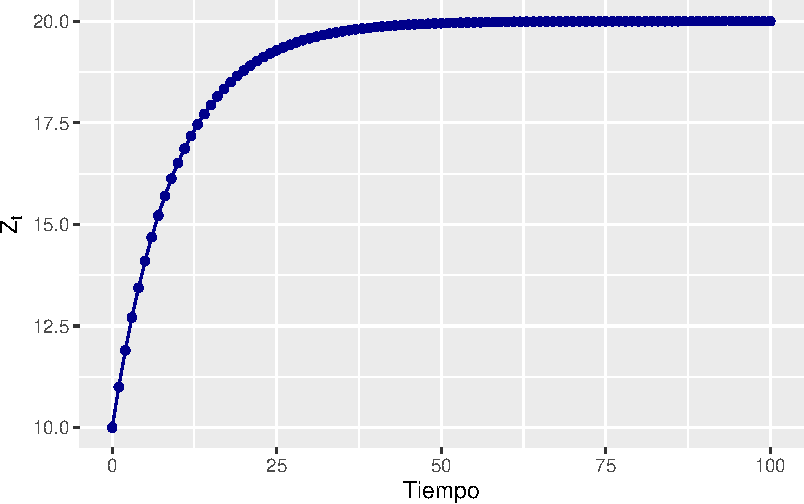
\includegraphics{index_files/figure-pdf/fig-fig21-1.pdf}

}

\end{figure}

\begin{Shaded}
\begin{Highlighting}[]
\FunctionTok{ggplot}\NormalTok{(,}\FunctionTok{aes}\NormalTok{(}\AttributeTok{x =}\NormalTok{ Tiempo, }\AttributeTok{y=}\NormalTok{Zt2))}\SpecialCharTok{+}
  \FunctionTok{geom\_line}\NormalTok{(}\AttributeTok{col=}\StringTok{"red4"}\NormalTok{)}\SpecialCharTok{+}
  \FunctionTok{geom\_point}\NormalTok{(}\AttributeTok{col=} \StringTok{"red4"}\NormalTok{)}\SpecialCharTok{+}
  \FunctionTok{labs}\NormalTok{(}\AttributeTok{y=}\FunctionTok{expression}\NormalTok{(Z[t]))}
\end{Highlighting}
\end{Shaded}

\begin{figure}[H]

\caption{\label{fig-fig22}Evolución del proceso dado por
\(Z_t =2-0.5Z_{t-1}\)}

{\centering 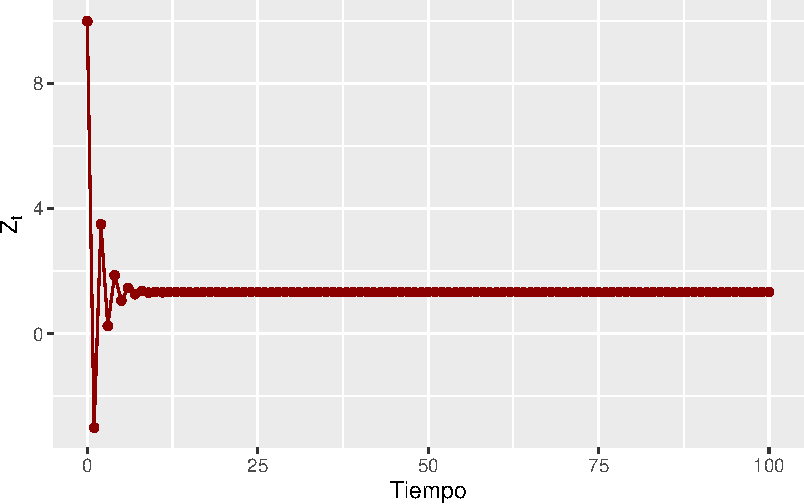
\includegraphics{index_files/figure-pdf/fig-fig22-1.pdf}

}

\end{figure}

\hypertarget{ecuaciones-en-diferencia-lineales-de-segundo-orden-y-de-orden-superior}{%
\subsubsection{Ecuaciones en Diferencia Lineales de Segundo Orden y de
orden
superior}\label{ecuaciones-en-diferencia-lineales-de-segundo-orden-y-de-orden-superior}}

Como un segundo caso a estudiar se ubica el caso de las Ecuaciones en
Diferencia Lineales de Segundo Orden y de orden superior. Primero, sea
una ecuación como la siguiente, la cual es lineal y de segundo orden, ya
que tiene asociado un término de \(Z_t\) rezagado dos periódos:

\begin{equation}\protect\hypertarget{eq-EDSO}{}{
Z_t = a_0 + a_1 Z_{t-1} + a_2 Z_{t-2}
}\label{eq-EDSO}\end{equation}

Donde \(t = \ldots, -2, -1, 0, 1, 2, \ldots\) y \(a_1, a_2 \neq 0\).
Reordenando la (Ecuación~\ref{eq-EDSO}) podemos escribir:

\begin{align}
Z*t - a_1 Z*{t-1} - a*2 Z*{t-2} & = a*0 \nonumber \\
Z_t - a_1 L Z*{t} - a*2 L^2 Z*{t} & = a_0 \nonumber \\
(1 - a_1 L - a_2 L^2)Z_t & = a_0
\end{align} \{\#eq-EDSOSOL\}

Así, la solución general propuesta para la (\textbf{?@eq-EDSOSOL}) es la
siguiente, la cual es una forma analóga a una Ecuación Lineal en
Diferencia de Primer Orden:

\begin{equation}\protect\hypertarget{eq-SOLGEN2}{}{
Z_t = \frac{a_0}{1 - a_1 - a_2} + s_1 g^t_1 + s_2 g^t_2
}\label{eq-SOLGEN2}\end{equation}

En donde \(s_1\) y \(s_2\) son constantes que se determinan mediante dos
condiciones iniciales --por lo que para resolver este tipo de ecuaciones
requerimos conocer dos condiciones iniciales--. Los valores de \(g_1\) y
\(g_2\) están relacionados con los coeficientes \(a_1\) y \(a_2\), de
esta forma:

\begin{equation}\protect\hypertarget{eq-a1}{}{
a_1 = g_1 + g_2
}\label{eq-a1}\end{equation}

\begin{equation}\protect\hypertarget{eq-a2}{}{
a_2  =  - g_1 g_2
}\label{eq-a2}\end{equation}

Lo anterior surge del siguiente procedimiento y recordando que siempre
es posible descomponer una ecuación cuadrática en expresiones como las
siguientes:

\begin{align}
(1 - a_1 L - a_2 L^2) & = (1 - g_1 L)(1 - g_2 L) \nonumber \\
& = 1 - g_1 L - g_2 L + g_1 g_2 L^2 \nonumber \\
& = 1 - (g_1 + g_2) L + g_1 g_2 L^2
\end{align} \{\#eq-eqcaracteristica\}

Donde se observa la equivalencia mostrada en (Ecuación~\ref{eq-a1}) y
(Ecuación~\ref{eq-a2}). Así, considerando la (Ecuación~\ref{eq-SOLGEN2})
tenemos que:

\begin{align}
(1 - a_1 L - a_2 L^2) Z_t & = (1 - g_1 L)(1 - g_2 L) Z_t \nonumber \\
& = a_0 + (1 - g_1 L)(1 - g_2 L) s_1 g^t_1 \nonumber \\
& = + (1 - g_1 L)(1 - g_2 L) s_2 g^t_2
\end{align}

Por lo tanto, buscamos que para que el proceso sea equivalente y podamos
interpretar que la (Ecuación~\ref{eq-SOLGEN2}) sea una solución general
deberá pasar lo siguiente:

\[
(1 - g_1 L) (1 - g_2 L) s_1 g^t_1 + (1 - g_1 L) (1 - g_2 L) s_2 g^t_2 = 0
\]

O, escrito de otra forma:

\[
(1 - g_1 L) s_1 g^t_1 = (1 - g_2 L) s_2 g^t_2 = 0
\]

Ahora determinemos cuáles son los valores \(g_1\) y \(g_2\) dados los
valores \(a_1\) y \(a_2\) que nos permitan determinar si el proceso será
convergente. Para ello debemos resolver la siguiente ecuación que se
deriva de la (\textbf{?@eq-eqcaracteristica}):

\[
1 - a_1 x - a_2 x^2 = (1 - g_1 x)(1 - g_2 x) = 0
\]

Donde, claramente existen dos raíces: \(x_1 = g^{-1}_1\) y
\(x_2 = g^{-1}_2\). Así, la solución estará dada por las raíces de la
ecuación característica:

\begin{align}
1 - a_1 x - a_2 x^2 & = 0 \nonumber \\
a_2 x^2 + a_1 x - 1 & = 0
\end{align} \{\#eq-POL2\}

Cuya solución es:

\[
x = \frac{- a_1 \pm \sqrt{a^2_1 + 4 a_2}}{2 a_2}
\]

Es importante distinguir tres diferentes casos en relación con las
raíces que surgen como solución de la (\textbf{?@eq-POL2}), estos son:

\textbf{Caso I}. Si \(a^2_1 + 4 a_2 > 0\), la (\textbf{?@eq-POL2})
proporcionará dos valores de raíces reales y distintos, eso es
\(x_1 = g^{-1}_1 \neq x_2 = g^{-1}_2\). Si por ahora suponemos que
\(|{g_1} < 1|\) y que \(|{g_2} < 1|\), entonces tendremos que:

\begin{align}
(1 - g*1 L)^{-1} (1 - g_2 L)^{-1} a_0 & = \left( \sum^{\infty}*{j = 0}{g^j*1 L^j} \right) \left( \sum^{\infty}*{j = 0}{g^j*2 L^j} \right) a_0 \nonumber \\
& = \left( \sum^{\infty}*{j = 0}{g^j*1} \right) \left( \sum^{\infty}*{j = 0}{g^j_2} \right) a_0 \nonumber \\
& = \frac{a_0}{(1 - g_1)(1 - g_2)} \nonumber \\
& = \frac{a_0}{1 - a_1 - a_2}
\end{align}

Esto último es el punto de equilibrio de la (Ecuación~\ref{eq-SOLGEN2});
considerando que \(|{g_1} < 1|\) y que \(|{g_2} < 1|\) --notemos que los
demás casos son divergentes, ya que la suma anterior nno connvergería--.
De esta forma la solución de la ecuación estará dada por:

\begin{equation}\protect\hypertarget{eq-Conver}{}{
\lim_{t \to \infty} Z_t = \frac{a_0}{1 - a_1 - a_2}
}\label{eq-Conver}\end{equation}

\textbf{Caso II}. Si \(a_1^2 + 4a_2 < 0\) en la (\textbf{?@eq-POL2}),
entonces las raíces serán números complejos conjugados, es decir:

\begin{align}
g_i^{-1} & = a \pm ib \\
g_i & = u \pm iv
\end{align}

Dichas raíces las podemos escribir en coordenadas polares como:

\begin{align}
g_1^{-1} & = r e^{i \theta} = r (cos(\theta) + i sen(\theta)) \\
g_2^{-1} & = r e^{-i \theta} = r (cos(\theta) - i sen(\theta))
\end{align}

Donde: \(r = \sqrt{u^2 + v^2}\), a esta expresión también se le conoce
como modulo. Alternativamente, podemos escribir que
\(r = \sqrt{g_1 g_2}\). La única condición es que \(r < 1\) para que el
proceso descrito en la (Ecuación~\ref{eq-SOLGEN2}) sea convergente.

Al igual que en el \textbf{Caso I}, el punto de equilibrio de la
ecuación se debería ubicar al rededor (Ecuación~\ref{eq-Conver}),
siempre que \(r < 1\), por lo que el factor que determina la
convergencia es el modulo, ya que si el modulo es mayor a 1, el proceso
será divergente, pero si es menor a 1 convergerá a
(Ecuación~\ref{eq-Conver}). Para ilustrar, el caso contrario es
divergente puesto que representa trayentorias senoidales (oscilatorias)
que sólo pueden converger si a medida que pasa el tiempo, las ondas son
menos amplias.

\textbf{Caso III}. Ahora revisemos el caso en el que
\(a_1^2 + 4a_2 = 0\), de esta forma las raíces serán identicas:

\[
g = g_1^{-1} = g_2^{-1} = \frac{-a_1}{2 a_2}
\]

Así, el punto de equilibrio será dado por la solución descrita como:

\begin{align}
(1 - g L)^2 Z*t & = a_0 \nonumber \\
Z_t & = \frac{a_0}{(1 - g L)^2} + s_1 g^t + s_2 t g^t \nonumber \\
& = a_0 \sum*{i = 0}^{\infty} (1 + i) g^j + s_1 g^t + s_2 t g^t
\end{align}

Donde la expresión amnterior es resultado de considerar el siguiente
procedimiento. Sea:

\begin{align}
f(g) & = \frac{1}{(1 - g)} \\
& = \sum\_{j = 0}^{\infty} g^j \nonumber
\end{align}

Por lo que si hacemos la primer derivada del la expresión anterior
tenemos que:

\begin{align}
f'(g) & = \frac{1}{(1 - g)^2} \nonumber \\
& = \sum*{j = 0}^{\infty} j g^{j-1} \nonumber \\
& = 0 + g^0 + 2 g^1 + 3 g^2 + \ldots \nonumber \\
& = \sum*{j = 0}^{\infty} (1 + j) g^j \nonumber
\end{align}

Ahora veámos un ejemplo de una Ecuación Lineal en Diferencia de Segundo
Orden. Supongamos la ecuación y el desarrollo siguientes:

\begin{align}
Z*t & = 3 + 0.9 Z*{t-1} - 0.2 Z\_{t-2} \nonumber \\
(1 - 0.9 L + 0.2 L^2) Z_t & = 3 \nonumber
\end{align}

La solución dada por una ecuación similar a la (\textbf{?@eq-POL2}),
obtendríamos la solución dada por las ecuaciones equivalentes a:

\begin{align}
1 - 0.9 x + 0.2 x^2 & = 0 \nonumber \\ - 0.2 x^2 + 0.9 x - 1 & = 0 \nonumber
\end{align}

De donde las raíces del polinomio característico \(x_1 = g_1^{-1}\) y
\(x_2 = g_2^{-1}\) se obtienen de la expresión dada por:

\begin{align}
x & = \frac{-0.9 \pm \sqrt{0.81 + (4)(-0.2)}}{(2)(-0.2)} \nonumber \\
& = \frac{0.9 \pm 0.1}{0.4} \nonumber
\end{align}

Dado que el componente \(a^2_1 + 4 a_2\) es positivo, obtendremos dos
raíces reales. Las raíces estarán dadas por \(x_1 = 2.5\) y
\(x_2 = 2.0\), de lo cual podemos determinar que \(g_1 = 0.4\) y
\(g_2 = 0.5\). De esta forma tenemos que \(|g_1| < 1\) y \(|g_2| < 1\),
así la ecuación converge a la expresión dada por las siguientes
expresiones:

\begin{align}
Z_t & = \frac{3}{1 - 0.9 L + 0.2 L^2} + s_1 (0.4)^t + s_2 (0.5)^t \nonumber \\
& = \frac{3}{1 - 0.9 + 0.2} + s_1 (0.4)^t + s_2 (0.5)^t \nonumber \\
& = \frac{3}{(1 - 0.4)(1 - 0.5)} + s_1 (0.4)^t + s_2 (0.5)^t \nonumber
\end{align}

Al final, la ecuación que describe la solución general será:

\[
z_t = 10 + s_1 (0.4)^t + s_2 (0.5)^t
\]

Para determinar los valores de \(s_1\) y \(s_2\) necesitamos obtener dos
valores iniciales de la ecuación para lo cual iniciaremos como \(t = 0\)
y luego obtenemos el valor de \(t = 1\), consideremos el valor de
\(Z_0 = 0\) y \(Z_1 = 50\):

\begin{align*}
Z_0 & = 10 + s_1(0.4)^0 + s_2(0.5)^0 \\
0 & = 10 + s_1 + s_2 \\
Z_1 & = 10 + s_1(0.4)^1 + s_2(0.5)^1 \\
50 & = 10 + 0.4 s_1 + 0.5 s_2
\end{align*}

Por lo que la solución es: \(s_1 = -450\) y \(s_2 = 440\), de donde
podemos expresar la ecuación como:

\begin{equation}\protect\hypertarget{eq-Ejem01}{}{
Z_t = 10 - 450(0.4)^t + 440(0.5)^t
}\label{eq-Ejem01}\end{equation}

La (Ecuación~\ref{eq-Ejem01}) anterior convergerá al valor de 10 cuando
\(t \rightarrow \infty\). Para ilustrar la trayectoria de esta ecuación
tomemos un cuadro similar al de los ejemplos anteriores. En la
Tabla~\ref{tbl-table2} y la Figura~\ref{fig-fig23} mostramos los
resultados de la trayectorua para 100 periodos.

\begin{Shaded}
\begin{Highlighting}[]
\NormalTok{t }\OtherTok{=} \FunctionTok{ts}\NormalTok{(}\FunctionTok{c}\NormalTok{(}\DecValTok{0}\SpecialCharTok{:}\DecValTok{100}\NormalTok{))}

\NormalTok{Zt}\OtherTok{=}\DecValTok{10{-}450}\SpecialCharTok{*}\NormalTok{(}\FloatTok{0.4}\SpecialCharTok{\^{}}\NormalTok{t)}\SpecialCharTok{+}\DecValTok{440}\SpecialCharTok{*}\NormalTok{(}\FloatTok{0.5}\SpecialCharTok{\^{}}\NormalTok{t)}

\NormalTok{lista }\OtherTok{=} \FunctionTok{c}\NormalTok{(}\DecValTok{1}\SpecialCharTok{:}\DecValTok{16}\NormalTok{, }\DecValTok{97}\SpecialCharTok{:}\DecValTok{101}\NormalTok{)}
\NormalTok{t1 }\OtherTok{=}\NormalTok{ t[lista]}
\NormalTok{Zt1}\OtherTok{=}\NormalTok{Zt[lista]}


\NormalTok{tabla1 }\OtherTok{=} \FunctionTok{data.frame}\NormalTok{(Tiempo1, Zt1)}
\FunctionTok{colnames}\NormalTok{(tabla1) }\OtherTok{\textless{}{-}} \FunctionTok{c}\NormalTok{(}\StringTok{"Tiempo"}\NormalTok{, }\StringTok{"$Z\_t =10{-}450(0.4)\^{}t+440(0.5)\^{}t$"}\NormalTok{)}

\FunctionTok{kable}\NormalTok{(tabla1, }\AttributeTok{format =} \StringTok{"pandoc"}\NormalTok{)}\SpecialCharTok{\%\textgreater{}\%}
  \FunctionTok{kable\_styling}\NormalTok{(}\AttributeTok{font\_size =} \DecValTok{10}\NormalTok{)}
\end{Highlighting}
\end{Shaded}

\hypertarget{tbl-table2}{}
\begin{longtable}[]{@{}ll@{}}
\caption{\label{tbl-table2}Un ejemplo de proceso de Ecuación de Segundo
Orden convengente}\tabularnewline
\toprule\noalign{}
Tiempo & \(Z_t =10-450(0.4)^t+440(0.5)^t\) \\
\midrule\noalign{}
\endfirsthead
\toprule\noalign{}
Tiempo & \(Z_t =10-450(0.4)^t+440(0.5)^t\) \\
\midrule\noalign{}
\endhead
\bottomrule\noalign{}
\endlastfoot
0 & 0.00000 \\
1 & 50.00000 \\
2 & 48.00000 \\
3 & 36.20000 \\
4 & 25.98000 \\
5 & 19.14200 \\
6 & 15.03180 \\
7 & 12.70022 \\
8 & 11.42384 \\
9 & 10.74141 \\
10 & 10.38250 \\
11 & 10.19597 \\
12 & 10.09987 \\
13 & 10.05069 \\
14 & 10.02565 \\
15 & 10.01294 \\
96 & 10.00000 \\
97 & 10.00000 \\
98 & 10.00000 \\
99 & 10.00000 \\
100 & 10.00000 \\
\end{longtable}

\begin{Shaded}
\begin{Highlighting}[]
\FunctionTok{ggplot}\NormalTok{(,}\FunctionTok{aes}\NormalTok{(}\AttributeTok{x =}\NormalTok{ t, }\AttributeTok{y=}\NormalTok{Zt))}\SpecialCharTok{+}
  \FunctionTok{geom\_line}\NormalTok{(}\AttributeTok{col=}\StringTok{"green4"}\NormalTok{)}\SpecialCharTok{+}
  \FunctionTok{geom\_point}\NormalTok{(}\AttributeTok{col=} \StringTok{"green4"}\NormalTok{)}\SpecialCharTok{+}
  \FunctionTok{labs}\NormalTok{(}\AttributeTok{y=}\FunctionTok{expression}\NormalTok{(Z[t]))}
\end{Highlighting}
\end{Shaded}

\begin{figure}[H]

\caption{\label{fig-fig23}Evolución del proceso dado por
\(Z_t =3+0.9Z_{t-1}-0.2Z_{t-2}\)}

{\centering 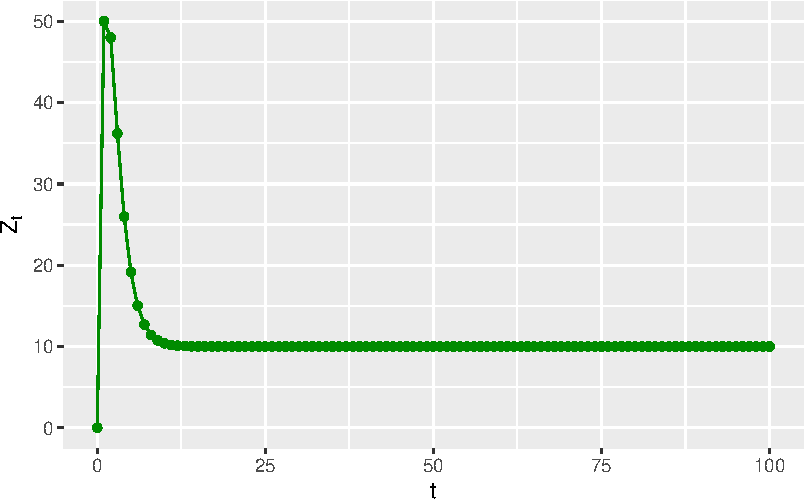
\includegraphics{index_files/figure-pdf/fig-fig23-1.pdf}

}

\end{figure}

Finalmente, discutiremos la solución para las Ecuaciones Lineales en
Diferencia de Orden \(p\), donde \(p \geq 2\). En general una ecuación
de este tipo se puede escribir como:

\begin{equation}\protect\hypertarget{eq-EDOP}{}{
Z_t = a_0 + a_1 Z_{t-1} + a_2 Z_{t-2} + \ldots + a_p Z_{t-p}
}\label{eq-EDOP}\end{equation}

Donde \(t = \ldots, -2, -1, 0, 1, 2, \ldots\) y \(a_p \neq 0\). La
(Ecuación~\ref{eq-EDOP}) se puede escribir como:

\begin{align}
Z*t - a_1 Z*{t-1} - a*2 Z*{t-2} - \ldots - a*p Z*{t-p} & = a_0 \nonumber \\
Z_t - a_1 L Z_t - a_2 L^2 Z_t - \ldots - a_p L^p Z_t & = a_0 \nonumber \\
(1 - a_1 L - a_2 L^2 - \ldots - a_p L^p) Z_t & = a_0
\end{align} \{\#eq-EDOP2\}

Por el Teorema Fundamental del Álgebra es posible escribir a la
(\textbf{?@eq-EDOP2}) como:

\begin{align}
(1 - g_1 L)(1 - g_1 L) \ldots (1 - g_p L) Z_t & = a_0
\end{align} \{\#eq-EDOP3\}

Utilizando la (\textbf{?@eq-EDOP2}) y la (\textbf{?@eq-EDOP3}) tenemos
que la solución general de una ecuación como la descrita en
(Ecuación~\ref{eq-EDOP}) se puede escribir como:

\begin{equation}\protect\hypertarget{eq-EDOPGEN}{}{
Z_t  =  \frac{a_0}{1 - a_1 - a_2 - \ldots - a_p} + s_1 g^t_1 + s_2 g^t_2 + \ldots + s_p g^t_p \\
}\label{eq-EDOPGEN}\end{equation}

\begin{align}
Z_t & = \frac{a_0}{(1 - g_1)(1 - g_1) \ldots (1 - g_p)} + s_1 g^t_1 + s_2 g^t_2 + \ldots + s_p g^t_p
\end{align} \{\#eq-EDOPGEN2\}

Donde \(s_1\), \(s_2\), \ldots, \(s_p\) son cosntantes que se determinan
utilizando \(p\) valores partículares de \(Z_t\), y la solución general
descrita en (Ecuación~\ref{eq-EDOPGEN}) y (\textbf{?@eq-EDOPGEN2})
implica encontrar \(p\) raíces: \(x_1 = g^{-1}_1\), \(x_2 = g^{-1}_2\),
\ldots, \(x_p = g^{-1}_p\) de los siguientes polinomios equivalentes:

\begin{align}
(1 - g_1)(1 - g_1) \ldots (1 - g_p) & = 0 \\
1 - a_1 x - a_2 x^2 - \ldots - a_p x^p & = 0 \\
a_p x^p + \ldots + a_2 x^2 + a_1 x - 1 & = 0
\end{align} \{\#eq-POLGEN\}

Antes de plantear la solución general, analicemos una solución patícular
cuando un conjunto de las \(p\) raíces, digamos un total de \(m\), son
iguales, es decir, cuando sucede que \(g_1 = g_2 = \ldots = g_m = g\)
(con \(1 < m \leq p\)). En este caso la solución general en la
(\textbf{?@eq-EDOPGEN2}) se escribe como:

\begin{align}
Z*t & = \frac{a_0}{(1 - g)^m(1 - g*{m+1}) \ldots (1 - g*p)} + s_1 g^t + s_2 t g^t + \ldots + s_m t^{m-1} g^t + s*{m+1} g^t*{m+1} + \ldots + s*{p} g^t\_{p}
\end{align} \{\#eq-EDOPGEN3\}

Definamos:

\[
f(g) = \frac{1}{1 - g} = \sum_{j = 0}^{\infty} g^j
\]

Si retomamos el método descrito parráfos arriba tenemos las siguientes
expresiones. Cuando \(m = 2\):

\[
f'(g) = \frac{1}{(1 - g)^2} = \sum_{j = 0}^{\infty} j g^{j-1} = \sum_{j = 0}^{\infty} (1 + j) g^j \nonumber
\]

En el otro extremo, cuando \(m = p\):

\[
f^{(p-1)}(g) = \frac{p-1}{(1 - g)^p} = \sum_{j = 0}^{\infty} \frac{(p-1+j)(p-2+j) \ldots (2+j)(1+j)}{(p-1)!} g^j
\]

Así, en el extremo cuando \(m = p\) la solución general podría estar
dada por:

\begin{align}
Z*t & = a_0 \sum*{j = 0}^{\infty} \frac{(p-1+j)(p-2+j) \ldots (2+j)(1+j)}{(p-1)!} g^j + g^t \sum\_{i = 0}^p s_i t^{i-1}
\end{align} \{\#eq-EDOPGEN4\}

Donde \(|{g} < 1|\), \(t = \ldots, -2, -1, 0, 1, 2, \ldots\). Para
finalizar esta sección, plantearemos la expresión de polinomio
característico que nos permitirá hacer el análisis de convergencia de
los procesos. Partamos de que la (\textbf{?@eq-POLGEN}) se puede
escribir como:

\begin{equation}\protect\hypertarget{eq-POLGEN2}{}{
(x^{-1})^p - a_1 (x^{-1})^{p-1} - a_2 (x^{-1})^{p-1} - \ldots - a_p = 0
}\label{eq-POLGEN2}\end{equation}

La (Ecuación~\ref{eq-POLGEN2}) permite interpretar las raíces del
polinomio característico de forma directa ya que \(x^{-1}_1 = g_1\),
\(x^{-1}_2 = g_2\), \ldots, \(x^{-1}_p = g_p\). Así, siempre que
\(p \geq 1\) en la (Ecuación~\ref{eq-EDOP}), diremos que el proceso
descrito en esa ecuación dará como resultado un proceso convergente si
se cumplen las dos condiciones (Ecuación~\ref{eq-COND1}) y
(Ecuación~\ref{eq-COND2}):

\begin{equation}\protect\hypertarget{eq-COND1}{}{
|a_p| < 1
}\label{eq-COND1}\end{equation}

\begin{equation}\protect\hypertarget{eq-COND2}{}{
a_1 + a_2 + \ldots + a_p < 1
}\label{eq-COND2}\end{equation}

Alternativamente, cuando las raíces son reales lo anterior es
equivalente a la (\textbf{?@eq-COND3}):

\begin{align}
|g_i| < 1
\end{align} \{\#eq-COND3\}

Para \(\forall i = 1, 2, \ldots, p\). Cuando la raíces son imaginarias,
las dos condiciones (Ecuación~\ref{eq-COND1}) y
(Ecuación~\ref{eq-COND2}) son equivalentes a la expresión
(\textbf{?@eq-COND4}):

\begin{align}
\sqrt{g_i g_j} = \sqrt{u^2 + v^2} < 1
\end{align} \{\#eq-COND4\}

Para \(\forall i \neq j\) y \(i, j = 1, 2, \ldots, p\). Cuando
\(g_1 = g_2 = \ldots = g_p = g\), la condición de la
(\textbf{?@eq-COND3}) se resume a que \(|g| < 1\). En resumen, las
condiciones descritas en (\textbf{?@eq-COND3}) y (\textbf{?@eq-COND4})
se puden ilustrar con un circulo unitario como el de la
Figura~\ref{fig-fig24} en que sí las raíces se ubican dentro de éste,
podemos decir que el proceso es convergente en el largo plazo.

\begin{Shaded}
\begin{Highlighting}[]
\NormalTok{x }\OtherTok{=} \FunctionTok{seq}\NormalTok{(}\SpecialCharTok{{-}}\DecValTok{1}\NormalTok{,}\DecValTok{1}\NormalTok{,}\FloatTok{0.001}\NormalTok{)}
\NormalTok{y }\OtherTok{=} \FunctionTok{sqrt}\NormalTok{(}\DecValTok{1}\SpecialCharTok{{-}}\NormalTok{x}\SpecialCharTok{\^{}}\DecValTok{2}\NormalTok{)}
\FunctionTok{par}\NormalTok{(}\AttributeTok{new =}\NormalTok{ T)}
\FunctionTok{plot}\NormalTok{(x,y, }\AttributeTok{type =} \StringTok{"line"}\NormalTok{, }\AttributeTok{ylim =} \FunctionTok{c}\NormalTok{(}\SpecialCharTok{{-}}\DecValTok{1}\NormalTok{,}\DecValTok{1}\NormalTok{), }\AttributeTok{col=}\StringTok{"red4"}\NormalTok{)}
\FunctionTok{par}\NormalTok{(}\AttributeTok{new =}\NormalTok{ T)}
\FunctionTok{plot}\NormalTok{(x,}\SpecialCharTok{{-}}\NormalTok{y, }\AttributeTok{type =} \StringTok{"line"}\NormalTok{, }\AttributeTok{ylim =} \FunctionTok{c}\NormalTok{(}\SpecialCharTok{{-}}\DecValTok{1}\NormalTok{,}\DecValTok{1}\NormalTok{), }\AttributeTok{ylab =} \StringTok{""}\NormalTok{, }\AttributeTok{col=}\StringTok{"red4"}\NormalTok{)}
\FunctionTok{abline}\NormalTok{(}\AttributeTok{v =} \DecValTok{0}\NormalTok{)}
\FunctionTok{abline}\NormalTok{(}\AttributeTok{h=}\DecValTok{0}\NormalTok{)}
\end{Highlighting}
\end{Shaded}

\begin{figure}[H]

\caption{\label{fig-fig24}Circulo unitario en el que se cumple que
\(|g_i|<1\) y \((g_i g_j)^{1/2} = (u^2 + v^2)^{1/2} < 1\)}

{\centering 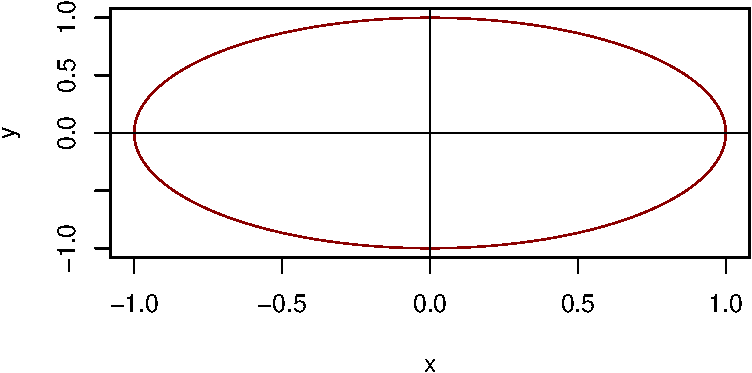
\includegraphics{index_files/figure-pdf/fig-fig24-1.pdf}

}

\end{figure}

\hypertarget{operador-de-rezago-l}{%
\subsection{Operador de rezago L}\label{operador-de-rezago-l}}

Denotemos, como se ha mencionado con anterioridad, con \(L\) al operador
de rezago, el cual nos permitirá construir una relación entre
diferencias y medias móviles como se verá más adelante en los procesos
univariados \(AR(p)\), \(MA(q)\) y, en general, \(ARIMA(p, d, q)\). Sean
\(X\), \(Y\) o \(Z\) variables con las que denotaremos a una serie de
tiempo (note que hasta el momento no hemos definido qué es una serie de
tiempo, no obstante no es necesario definirla para hacer uso del
operador).

En esta sección resumiremos algunas propiedades usadas en el capítulo y
en capítulos más adelante. Así, si a dicha serie le aplicamos el
operador rezago antes definido, el resultado deberá ser que cada uno de
los valores de la serie es retardado o regresado un período. Es decir:

\begin{equation}\protect\hypertarget{eq-Lag1}{}{
L Z_t = Z_{t-1}
}\label{eq-Lag1}\end{equation}

De esta forma, si aplicamos el operador rezago \(L\) a la nueva serie de
tiempo dada por \(Z_{t-1}\) podemos obtener \(Z_{t-2}\), haciendo uso de
la (Ecuación~\ref{eq-Lag1}) podemos obtener:

\[
L Z_{t-1} = L(L Z_t) = L^2 Z_t = Z_{t-2}
\]

Mediante una generalización podemos obtener:

\[
L^k Z_t = Z_{t-k}
\]

Para \(k = \ldots, -2, -1, 0, 1, 2, \ldots\). Así, para \(k = 0\)
obtenemos la identidad dado que \(L^0 Z_t = Z_t\), de tal forma que
siempre asumiremos que \(L^0 = 1\). En otro caso, cuando \(k > 0\) a la
serie de tiempo a la cual se le aplique el operador rezago \(L\) se le
deberá aplicar un rezago de \(k\) periodos a cada uno de los elementos
de la serie. Por el contrario, cuando \(k < 0\) el operador rezago
significa que se deberá adelantar \(|k|\) veces a cada elemento de la
serie. Por ejemplo, \(L^{-3} Z_t = Z_{t+3}\).

Las reglas descritas en lo subsecuente se mantienen indistintamene
cuando aplican para el caso de rezagar como para cuando se adelanta una
serie. Como primera propiedad tomemos a la siguiente propiedad:

\[
L^{m} Z_{t-n} = L^{m} (L^{n} Z_{t}) = L^{m + n} Z_{t} = Z_{t-(n + m)}
\]

De lo anterior podemos inferir el siguiente resultado:

\[
\Delta Z_{t} = Z_{t} - Z_{t-1} = (1 - L) Z_{t}
\]

En el caso de la diferencia de órden cuatro o cuarta diferencia se puede
expresar como:

\begin{equation}\protect\hypertarget{eq-Diff4}{}{
\Delta_{4} Z_{t} = Z_{t} - Z_{t-4} = (1 - L^4) Z_{t}
}\label{eq-Diff4}\end{equation}

Al respecto, vale la pena aclarar que en ocaciones se hará uso de una
notación alternativa dada por: \(\Delta^k\) o \(\Delta_k\), donde
\(k = 1, 2, 3, \ldots\), indistintamente, ya que en ambos casos se
referirá a una diferencia de orden \(k\). Esta notación resulta de gran
utilidad cuando se quiere comparar periodos equivalentes como, por
ejemplo, el mismo trimestre pero de un año anterior. De forma similar,
para el caso de logarítmos podemos escribir a la
(Ecuación~\ref{eq-Diff4}) como:

\[
\Delta^{4} ln(Z_{t}) = \Delta_{4} ln(Z_{t}) = ln(Z_{t}) - ln(Z_{t-4}) = (1 - L^4) ln(Z_{t})
\]

Para el caso de una serie de tiempo que se le ha transformado mediante
medias móviles, digamos de \(4\) periodos, podemos escribirla como:

\[
Zs_{t} = \frac{1}{4}(Z_{t} + Z_{t-1} + Z_{t-2} + Z_{t-3}) = \frac{1}{4}(1 + L + L^2 + L^3)Z_{t}
\]

Una generalización del anterior caso puede ser escrito como un polinomio
de orden \(p\) con el operador rezago \(L\) dado como:

\begin{align}
\alpha(L) Z*{t} & = (1 - \alpha_1 L - \alpha_2 L^2 - \ldots - \alpha_p L^p) Z*{t} \nonumber \\
& = Z*{t} - \alpha_1 Z*{t-1} - \alpha*2 Z*{t-2} - \ldots - \alpha*p Z*{t-p}
\end{align} \{\#eq-Ecp1\}

Donde \(\alpha_i\) puede ser remplazada por cualquier constante \(a_i\),
con \(i = 1, 2, 3, \ldots\), para escribir ecuaciones como las
anteriores. Adicionalmente, podemos decir que la (\textbf{?@eq-Ecp1}) es
una generalización del caso de medias móviles, el cual admite una
poderación distinta para cada uno de los elementos rezagados.

Existe la posibilidad de operar más de un polinomio a la vez. Para
múltiples polinomios (digamos, los polinomios \(\alpha(L)\) y
\(\beta(L)\)) podemos escribir el siguiente resultado:

\[
\alpha(L) \beta(L) = \beta(L) \alpha(L)
\]

Tales polinomios del operador rezago también son llamados \emph{filtros
lineales}. A manera de ejemplo tomemos el siguiente caso de diferencias
para una serie de \(Z_t\):

\[
\Delta Z_{t} = (1 - L) Z_{t} = Z_{t} - Z_{t-1}
\]

y un proceso de medias móviles para la misma serie de \(Z_t\):

\[
Zs_{t} = \frac{1}{4}(1 + L^1 + L^2 + L^3) Z_{t} = \frac{1}{4}(Z_{t} + Z_{t-1} + Z_{t-2} + Z_{t-3})
\]

De tal forma que el producto de ambos procesos se puede escribir como:

\[
(1 - L) \times \frac{1}{4}(1 + L^1 + L^2 + L^3) Z*{t} = \frac{1}{4}(1 - L^4) Z*{t}
\]

Es decir, que el producto de dos polinomios, uno de diferencias y otro
más de medias móviles, resulta en uno de diferencias pero de mayor
grado, en este caso de grado 4.


\printbibliography


\end{document}
